\documentclass[11pt,a4paper]{article}
\usepackage[T1]{fontenc}
\usepackage[utf8]{inputenc}
\usepackage[margin=24mm,headheight=15pt,footskip=15mm]{geometry}
\usepackage{amsmath,amsthm,amssymb,mathtools}
\IfFileExists{newtxtext.sty}{\usepackage{newtxtext,newtxmath}}{\usepackage{lmodern}\usepackage{mathptmx}}
\usepackage{graphicx,booktabs,tabularx,array,longtable,multirow}
\usepackage[table]{xcolor}
\usepackage{tikz}
\usetikzlibrary{arrows.meta,positioning,calc,shapes.geometric,fit,backgrounds,decorations.pathreplacing}
\usepackage{tcolorbox}
\tcbuselibrary{breakable,skins}
\usepackage{enumitem}
\usepackage{microtype}
\usepackage{fancyhdr}
\usepackage{titlesec}
\usepackage{hyperref}
\usepackage{needspace}
\hypersetup{colorlinks=true,linkcolor=tealdark,urlcolor=tealdark,citecolor=tealdark,pdftitle={The Intrinsic--Selected Hierarchy of UNNS Arithmetic Dynamics},pdfauthor={UNNS Research Collective},pdfsubject={Arithmetic transition systems, graph geometry, intrinsic history entropy and autonomous selection}}
\definecolor{tealdark}{HTML}{106A75}
\definecolor{ink}{HTML}{182B39}
\definecolor{ochre}{HTML}{B8862A}
\definecolor{pale}{HTML}{EAF4F3}
\definecolor{slate}{HTML}{627784}
\definecolor{ltline}{HTML}{C7DADA}
\color{ink}
\titleformat{\section}{\Large\bfseries\color{tealdark}}{\thesection}{0.8em}{}
\titleformat{\subsection}{\large\bfseries\color{tealdark}}{\thesubsection}{0.8em}{}
\titleformat{\subsubsection}{\normalsize\bfseries}{\thesubsubsection}{0.7em}{}
\titlespacing*{\section}{0pt}{2.4ex plus 1ex minus .5ex}{1.2ex}
\titlespacing*{\subsection}{0pt}{2ex plus .5ex minus .5ex}{.7ex}
\newtheorem{theorem}{Theorem}[section]
\newtheorem{proposition}[theorem]{Proposition}
\newtheorem{lemma}[theorem]{Lemma}
\newtheorem{corollary}[theorem]{Corollary}
\theoremstyle{definition}\newtheorem{definition}[theorem]{Definition}
\newtheorem{remark}[theorem]{Remark}
\newtheorem{observation}[theorem]{Observation}
\newcommand{\N}{\mathbb N}
\newcommand{\PP}{\mathcal P}
\newcommand{\A}{\mathcal A}
\newcommand{\G}{\mathfrak G}
\newcommand{\NB}{\mathrm{NB}}
\newcommand{\supp}{\operatorname{supp}}
\newcommand{\Und}{\operatorname{Und}}
\newcommand{\tr}{\operatorname{tr}}
\newcommand{\diam}{\operatorname{diam}}
\newcommand{\iso}{\cong}
\newcommand{\sel}{\sigma}
\providecommand{\vv}{}
\renewcommand{\vv}{\mathbf v}
\newcommand{\proj}{\pi}
\setlist[itemize]{leftmargin=*,topsep=3pt,itemsep=1.5pt}
\setlist[enumerate]{leftmargin=*,topsep=3pt,itemsep=1.5pt}
\newtcolorbox{takeaway}[1][]{colback=pale,colframe=tealdark,boxrule=.8pt,arc=2pt,left=9pt,right=9pt,top=7pt,bottom=7pt,breakable,#1}
\newtcolorbox{scopebox}[1][]{colback=white,colframe=ochre,boxrule=.9pt,arc=2pt,left=9pt,right=9pt,top=7pt,bottom=7pt,breakable,#1}
\pagestyle{fancy}\fancyhf{}\fancyhead[L]{\footnotesize\color{slate}UNNS MATHEMATICAL FOUNDATIONS}\fancyhead[R]{\footnotesize\color{slate}INTRINSIC STRUCTURE / SELECTED DYNAMICS}\fancyfoot[C]{\color{slate}\thepage}\renewcommand{\headrulewidth}{0.35pt}
\renewcommand{\arraystretch}{1.19}
\begin{document}
\begin{titlepage}
\thispagestyle{empty}
\vspace*{13mm}
{\color{tealdark}\sffamily\bfseries\large UNNS MATHEMATICAL FOUNDATIONS \hfill RESEARCH SYNTHESIS 01}\par
\vspace{7mm}\noindent\color{ochre}\rule{\textwidth}{1.8pt}\par
\vspace{23mm}
{\color{ink}\Huge\bfseries The Intrinsic--Selected\\[5pt] Hierarchy of UNNS\\[5pt] Arithmetic Dynamics\par}
\vspace{13mm}
{\color{tealdark}\Large Arithmetic Transitions, Reversible Graph Geometry,\\ Intrinsic History Entropy, and Autonomous Selectors\par}
\vspace{20mm}
{\large UNNS Research Collective\\[5pt]\normalsize Synthesis and conceptual formalization based on four mathematical manuscripts\par}
\vspace{11mm}
{\color{slate}Version 1.4 \quad $\cdot$ \quad 14 November 2026\\ Source-anchored mathematical synthesis; no frozen source release modified\par}
\vfill
\begin{takeaway}
\textbf{Central thesis.} The complete legal arithmetic transition relation determines an all-branch reversible graph without prescribing a trajectory. Its geometry is independent of autonomous selection, while its nonbacktracking history spaces yield intrinsic graph-derived spectral and entropy quantities. MAXPP, ADJ4, and other selectors are additional dynamical grammars whose distinct invariants must be evaluated relative to their explicitly stated rules.
\end{takeaway}
\vspace{9mm}
\noindent\small\textbf{Scope of originality.} This paper contributes a clarified hierarchy, an invariant taxonomy, formal separation statements, a self-contained worked doubling-distance proof, and a research programme. Its major geometric, symbolic, spectral, and return theorems are attributed to the four source manuscripts. The architectural classification is not presented as a newly proved theorem of physical universality.\par
\end{titlepage}
\setcounter{page}{1}
\begin{abstract}
The arithmetic transformation $T_N(x)=x(N+1)^2/N$, defined on positive integers with $N\mid x$, gives rise to several mathematically distinct objects that share a common transition law but differ in the extra structure they retain or impose. We distinguish: (I) the complete labelled arithmetic transition system; (II) the undirected all-branch arithmetic graph and its integer-labelled metric geometry; (III) nonbacktracking history dynamics derived from the graph without a priority selector; and (IV) autonomous selected dynamics obtained by imposing a state-dependent choice of one legal branch. This separation provides a rigorous interpretation of the established results of the Geometry, Prime-Valuation, Autonomous Aperiodicity, and Graph Entropy manuscripts. We give a detailed proof that the sharp doubling-distance constant is $5$, deduce the selector independence of the unselected graph, and explain the distinction between abstract graph invariants and invariants of an arithmetic-labelled graph. We derive the arithmetic--topology--entropy identity for a family of arithmetic book graphs and contrast unbounded finite-subgraph history entropy with zero-entropy Sturmian behaviour under MAXPP. We add a third distinction, between structure, its lower-dimensional representation and a selected trajectory, and prove a sharp criterion for when a finite prime-valuation projection retains branch legality, supported by exact visual counterexamples. Finally, we discuss what is and is not meant by intrinsic structure, identify which mathematical decisions enter at each layer, compare the hierarchy with standard graph and dynamical constructions, and formulate testable research directions. No new physical constant, universal graph invariance across different generating rules, or equivalence of separate UNNS grammars is asserted.
\end{abstract}
\vspace{3mm}
\noindent\textbf{Keywords:} arithmetic transition system; labelled infinite graph; graph metric; prime valuations; scaling; nonbacktracking shift; Ihara--Bass theory; Sturmian dynamics; autonomous selectors; UNNS Substrate.\\
\textbf{Mathematical domains:} number theory, graph theory, symbolic dynamics, arithmetic dynamics, spectral graph theory.
\setcounter{tocdepth}{1}\tableofcontents
\newpage
\section{Introduction: what is intrinsic, and to what?}
\label{sec:intro}
A mathematical result about an infinite graph and a result about a selected orbit through that graph answer different questions. The former concerns a structure fixed once its vertices and edges are defined. The latter concerns a function---or more generally a trajectory grammar---that chooses a successor according to additional rules. Confusing these levels can make an exact structural theorem appear to be the outcome of a carefully engineered orbit. Conversely, calling every dynamical constant an invariant of the whole structure hides its dependence on a specific selector.

The UNNS arithmetic transition is simple enough to make this distinction exact. Let $\N=\{1,2,3,\ldots\}$, and define, whenever $N\mid x$,
\begin{equation}\label{eq:T}
T_N(x)=\frac{x(N+1)^2}{N}.
\end{equation}
The complete relation consisting of \emph{all} such legal moves produces a connected, locally finite graph with sharply bounded arithmetic distances. The same graph supports a well-defined nonbacktracking-history shift, whose finite-subgraph entropy capacity is unbounded. But selecting just one prime branch at a time under MAXPP produces a zero-entropy Sturmian itinerary, while the distinct ADJ4 priority grammar yields a certified expanding selected-return law. The statements are compatible because they concern different objects derived from the same transition relation \cite{geometry,prime,adj,entropy}.

Our thesis is therefore not simply that ``geometry comes before dynamics.'' It is more precise: the transition rule first determines a labelled directed relation, and the all-branch undirected graph is determined once the reversible-edge convention is declared. The graph and its integer labels then support different classes of invariants. A graph-history shift uses a uniform path rule and no priority selector. A deterministic selector is a new function on the legal branches and must be investigated as an additional system.

\begin{takeaway}
\textbf{Structural classification.} The primary arithmetic data are the legal partial maps $\{T_N\}$. The all-branch graph $G$ is a determined realization of these maps. Graph geometry and graph-derived history entropy are independent of the choice of an autonomous trajectory selector. MAXPP and ADJ4 define secondary selected systems with their own mathematical invariants.
\end{takeaway}

\begin{scopebox}
\textbf{Revision note (v1.4).} This release is typographical and editorial: cross-reference labels are written explicitly so that definitions, propositions and corollaries are named correctly in every build; the image attribution is completed; and one plot label is moved. No mathematical statement changes. Version 1.3 supplied the missing visual evidence in Section~\ref{sec:projection}: a credited planar $E_8$ image and two exact UNNS diagrams recording valuation collisions, legal branch translations, and projection-created shortcuts. The mathematical results and prior releases remain intact. Version 1.2 added Section~\ref{sec:projection}, which separates the arithmetic structure from its lower-dimensional representation and from a selected trajectory, with an E8 comparison that is methodological only and an exact proposition on finite prime-valuation projections. It also carries the v1.1 corrections: the legal-selector domain now includes branch $N=1$; the general-$x$ book-vertex distinctness argument and the transfer of the cubic from $F_m$ to $F(x)$ are written out; reference types are corrected; and the cycle results are credited to the frozen U3 and U3-COR releases. Versions 1.0 and 1.1 and all source manuscripts remain unchanged.
\end{scopebox}

\subsection{Source base and status of claims}
The mathematical inputs are the four standalone source manuscripts: \emph{Geometry and Metric Structure of the UNNS Arithmetic Graph}, v1.4 \cite{geometry}; \emph{Autonomous Prime-Valuation Dynamics and Symbolic Complexity in the UNNS Substrate}, v1.2 \cite{prime}; \emph{Autonomous Aperiodicity in the UNNS Substrate: An Expanding Arithmetic Return Theorem}, v2.7 \cite{adj}; and \emph{Intrinsic Symbolic Dynamics and Entropy of Arithmetic Graphs}, v1.5 \cite{entropy}. We also use the extended synthesis v1.3.2 \cite{synthesis} and a dedicated note giving an elementary doubling-distance proof \cite{doublingnote}.

Throughout we distinguish three evidence labels. \textbf{Source theorem} denotes a result proved in a cited manuscript; \textbf{derived statement} denotes a consequence proved here from specified inputs; and \textbf{research interpretation} denotes a proposed organizing principle or a question for future investigation. The algebraic and geometric results below do not require rerunning the source verification packages; where a source theorem is computer-assisted, we say so.

\subsection{Contributions of this paper}
The paper provides a unified formal setting for the four manuscripts; a taxonomy of graph-theoretic, arithmetic-labelled, history-space, and selector-dependent invariants; an explicit selector-independence proposition; a fully written proof of the sharp doubling-distance constant; a concise derivation of the arithmetic--topology--entropy identity; a distinction between uniform nonbacktracking admissibility and autonomous branch choice; a projection principle separating structure, representation and selection, with a proof characterizing precisely when a finite prime-valuation projection retains branch legality and with exact visual examples; and a programme for comparing intrinsic structure with selection effects. This is a synthesis and conceptual formalization, not a claim that every previously established theorem is reproved in full here.

\section{The transition system and the all-branch graph}
\label{sec:base}
\begin{definition}[Arithmetic transition system]\label{def:A}
Let $D_N=N\N$ for every $N\in\N$. The \emph{UNNS arithmetic transition system} is the family of partial maps
\begin{equation}\label{eq:A}
\A=\bigl(\N,\{T_N:D_N\longrightarrow\N\}_{N\geq1}\bigr),\qquad
T_N(x)=x\frac{(N+1)^2}{N}.
\end{equation}
Equivalently, it is the labelled directed relation
$\mathcal R=\{(x,N,T_N(x)):x\in\N,\ N\mid x\}$.
\end{definition}

The legality threshold is part of the definition. A branch parameter $N$ is not arbitrary at a state $x$; it may act only when $N\mid x$. The labels distinguish transitions even before any orientation or metric is forgotten.

\begin{definition}[All-branch arithmetic graph]\label{def:G}
The \emph{reversible arithmetic graph} is the simple undirected graph
\begin{equation}\label{eq:G}
G=(\N,E),\qquad
E=\bigl\{\{kN,k(N+1)^2\}:k,N\in\N\bigr\}.
\end{equation}
Every legal forward transition contributes one unoriented edge; no branch is prioritized or omitted.
\end{definition}

\begin{proposition}[Determination and selector independence]\label{prop:selectorfree}
Fix the family $\{T_N\}_{N\ge1}$ and the convention in Definition~\ref{def:G}. Then $E(G)$, the metric $d_G$, and every property computed solely from $G$ are determined without specifying a function that selects a legal branch at any vertex. Two selectors acting on the same family $\{T_N\}$ have the same ambient graph $G$, whether or not their selected trajectories intersect.
\end{proposition}
\begin{proof}
Each pair in $E(G)$ is obtained by taking an arbitrary legal input $x=kN$ and its image $T_N(x)=k(N+1)^2$. Conversely every legal pair has this form. Hence the set $E(G)$ is fixed by the transition relation and the instruction to include all such pairs, independently of any selector. The graph metric and graph-derived quantities are functions of this fixed edge set. A selector changes only which of the already legal directed edges its trajectory traverses.
\end{proof}

\begin{remark}[Scope of the proposition]
The result is logical rather than difficult: an object defined using all legal branches does not depend on a subsequently imposed choice among those branches. It does \emph{not} say that graph geometry is independent of changes to $T_N$, the admissible branch family, orientation conventions, edge weights, or integer labelling. Those are different mathematical questions.
\end{remark}

\subsection{A one-to-one correspondence between edge ratios and branch labels}
Set
\begin{equation}\label{eq:rN}
r_N=\frac{(N+1)^2}{N}=N+2+\frac1N.
\end{equation}
Then $r_1=4$ and $r_N$ is strictly increasing. Because $\gcd(N,(N+1)^2)=1$, the ratio $y/x$ of any upward edge $x<y$ is in lowest terms exactly $(N+1)^2/N$. Thus every upward edge has a unique legal branch label $N$ (Geometry, Lemma 2.4) \cite{geometry}. This property makes the passage from labelled moves to the unlabelled graph unusually transparent; one can recover the label from the arithmetic values of the endpoints, but not from the abstract isomorphism class of the graph alone.

\subsection{A hierarchy of derived objects}
\begin{figure}[htbp]
\centering
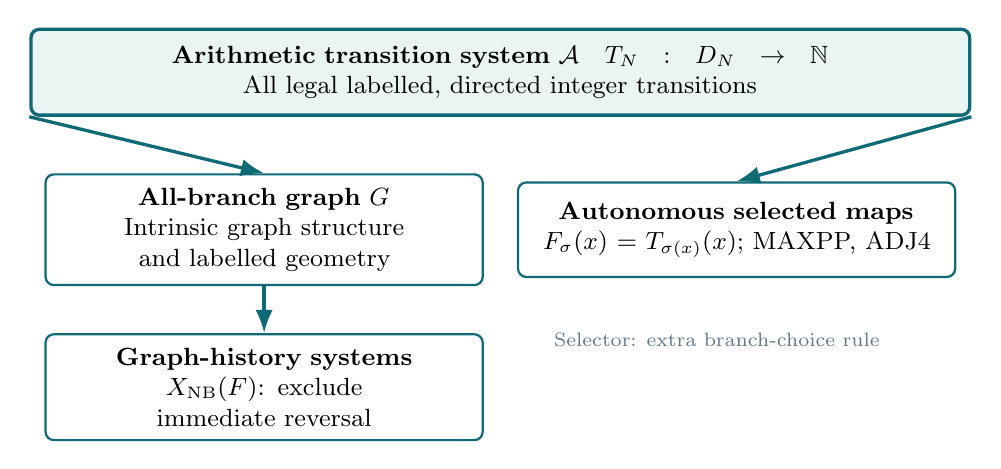
\begin{tikzpicture}[>=Latex, every node/.style={align=center},font=\small]
\tikzset{root/.style={draw=tealdark,rounded corners=3pt,very thick,fill=pale,text width=11.5cm,minimum height=1.05cm,inner sep=6pt},sub/.style={draw=tealdark,rounded corners=3pt,thick,fill=white,text width=5.2cm,minimum height=1.2cm,inner sep=5pt}}
\node[root] (ar) at (0,0) {\textbf{Arithmetic transition system $\mathcal A$}\quad $T_N:D_N\to\N$\\ All legal labelled, directed integer transitions};
\node[sub] (gr) at (-3.0,-2.0) {\textbf{All-branch graph $G$}\\ Intrinsic graph structure and labelled geometry};
\node[sub] (ss) at (3.0,-2.0) {\textbf{Autonomous selected maps}\\ $F_\sigma(x)=T_{\sigma(x)}(x)$; MAXPP, ADJ4};
\node[sub] (hs) at (-3.0,-4.0) {\textbf{Graph-history systems}\\ $X_{\NB}(F)$: exclude immediate reversal};
\draw[->,very thick,tealdark] (ar.south west) -- (gr.north);
\draw[->,very thick,tealdark] (ar.south east) -- (ss.north);
\draw[->,very thick,tealdark] (gr.south) -- (hs.north);
\node[font=\scriptsize,color=slate] at (2.75,-3.4) {Selector: extra branch-choice rule};
\end{tikzpicture}
\caption{Object hierarchy. The autonomous selectors are derived from the directed transition system, not from a freely chosen walk on the undirected graph. Nonbacktracking history dynamics is induced by the reversible graph after imposing the uniform exclusion of immediate edge reversal.}
\label{fig:hierarchy}
\end{figure}

Graph-history dynamics and autonomous selected dynamics have different mathematical roles. The nonbacktracking shift counts alternative reversible paths; MAXPP and ADJ4 evolve forward by a \emph{single selected legal transition} at each step. The graph may contain inverse edges and cycles even though the forward arithmetic is strictly increasing.

\section{The valuation law: exact additive coordinates}
\label{sec:valuation}
For each prime $p$, write $v_p(x)$ for the exponent of $p$ in the factorization of $x$. The following result is common to the arithmetic transition system and all derived grammars.

\begin{theorem}[Valuation law; source theorem]\label{thm:valuation}
For every legal transition $N\mid x$ and every prime $p$,
\begin{equation}\label{eq:valuation}
v_p(T_N(x))=v_p(x)+2v_p(N+1)-v_p(N).
\end{equation}
The step $T_N$ is legal at $x$ exactly when $v_p(x)\ge v_p(N)$ for every prime $p$.
\end{theorem}
\begin{proof}
On positive rationals, $v_p$ is additive under multiplication and changes sign under inversion. Apply it to $T_N(x)=x(N+1)^2N^{-1}$. The second assertion is the prime-factor criterion for divisibility.
\end{proof}

Let $\mathbf v(x)=(v_p(x))_p$ and set
\begin{equation}\label{eq:tau}
\boldsymbol\tau_N=(2v_p(N+1)-v_p(N))_p.
\end{equation}
Then a legal step is the translation $\mathbf v(x)\mapsto\mathbf v(x)+\boldsymbol\tau_N$ on a restricted domain of the nonnegative, finitely supported exponent lattice. The branch parameter enters through a fixed integer vector, while the current state enters through the legality thresholds. Multiplication and integer divisibility are therefore represented by lattice translation and coordinate inequalities.

\begin{proposition}[Injectivity of the translation label]
The map $N\mapsto\boldsymbol\tau_N$ is injective.
\end{proposition}
\begin{proof}
The vector $\boldsymbol\tau_N$ is the complete prime-valuation vector of the positive rational $r_N=(N+1)^2/N$. A positive rational is uniquely determined by its prime valuations. Since $N\mapsto r_N$ is strictly increasing, equal vectors imply equal parameters.
\end{proof}

\subsection{Strict forward growth is a consequence, not a choice}
For $N\ge1$ we have $r_N\ge4$, with equality only when $N=1$; for $N\ge2$, $r_N\ge9/2$. Thus every legal forward step is strictly increasing, and a directed orbit cannot contain a cycle. If all selected branches satisfy $N\ge2$, then $x_{t+1}\ge(9/2)x_t$. These growth bounds are properties of the forward law. They say nothing about whether a \emph{symbolic itinerary} of branch labels is eventually periodic.

\subsection{From one-step legality to a prescribed finite history}
Let $w=(N_0,\ldots,N_{\ell-1})$ be a proposed finite word of branches and define the rational partial products
\begin{equation}\label{eq:partials}
R_0=1,\qquad R_j=\prod_{i=0}^{j-1}\frac{(N_i+1)^2}{N_i},\quad 1\le j\le\ell.
\end{equation}
Write $\operatorname{den}(r)$ for the positive reduced denominator of a rational number $r$ and let
\begin{equation}\label{eq:K}
K(w)=\operatorname{lcm}\bigl(\operatorname{den}(R_0),\ldots,\operatorname{den}(R_\ell)\bigr).
\end{equation}
\begin{lemma}[Whole-history anchor criterion; derived statement]\label{lem:history}
The branch word $w$ is executable from an initial integer $x$ if and only if $K(w)\mid x$.
\end{lemma}
\begin{proof}
If the word executes, then its successive states are the integers $xR_j$, so every reduced denominator of $R_j$ divides $x$. Hence $K(w)\mid x$. Conversely, if $K(w)\mid x$ then each $xR_j$ is an integer. The relation $xR_{j+1}=xR_j(N_j+1)^2/N_j$, together with $\gcd(N_j,(N_j+1)^2)=1$, implies that $N_j\mid xR_j$. Thus every consecutive move is legal.
\end{proof}

This criterion is not a selector: it tests whether a \emph{given} word is admissible. It also illustrates a bridge to the separate GIG-I study of finite-history admissibility. We do not identify the homology of that programme with the graph-cycle homology considered below.

\section{Intrinsic metric geometry of the all-branch graph}
\label{sec:geometry}
Geometry v1.4 proves the stated connectivity, degree, and metric laws, and consolidates the corrected cycle results \cite{geometry}. Their original release provenance is more specific: U3 established triangle-freeness and odd girth $5$; U3-COR corrected the girth to $4$ \cite{u3,u3cor}. The four-cycle $2\sim8\sim36\sim9\sim2$ witnesses girth at most $4$; excluding triangles gives the matching lower bound. We state these results as invariants of the \emph{specified graph}, not as properties of an autonomous selector.

\begin{theorem}[Geometric result inventory; source theorems]\label{thm:geom}
Let $d=d_G$ be the unweighted graph distance in $G$. Then
\begin{equation}\label{eq:distances}
\sup_{n\ge1}d(n,n+1)=6,\qquad
\sup_{n\ge1}d(n,2n)=5,\qquad
\sup_{n\ge1}d(n^2,(n+1)^2)=5.
\end{equation}
Moreover
\begin{equation}\label{eq:degree}
\deg_G(x)=\tau(x)+\#\{q\ge2:q^2\mid x\},
\end{equation}
$G$ is connected, triangle-free with girth $4$ (U3-COR) and odd girth $5$ (U3), every prime has degree $2$, and no vertex has degree $3$ \cite{geometry,u3,u3cor}.
\end{theorem}

The three suprema in \eqref{eq:distances} are \emph{arithmetically specified distance invariants}, not invariant under arbitrary permutations of vertex labels. Their meaning depends on the distinguished relations $n\mapsto n+1$, $n\mapsto 2n$, and $n\mapsto n^2,(n+1)^2$. By contrast, girth and local degree are invariants of the unlabelled graph under graph isomorphism.

\subsection{Why the neighbourhood structure is arithmetic}
There are exactly $\tau(x)$ upward neighbours, one for each divisor $N\mid x$, since $r_N$ is strictly increasing. There is one downward neighbour for each $q\ge2$ with $q^2\mid x$: the inverse of the $N=q-1$ move. No upward neighbour can equal a downward neighbour since upward moves strictly increase. This proves the degree formula \eqref{eq:degree} directly.

\begin{corollary}[Non-homogeneity of the unlabelled graph]\label{cor:nonhom}
The graph $G$ is not vertex-transitive.
\end{corollary}
\begin{proof}
The degree of $1$ is $1$, whereas the degree of a prime is $2$. Vertex-transitivity would force all vertex degrees to coincide.
\end{proof}

This distinguishes the arithmetic graph from many conventional Cayley graphs of groups: although both carry intrinsic path metrics, $G$ has nonuniform degrees and no underlying group action is asserted.

\subsection{Scaling is a graph map, not generally a symmetry}
If $\{a,b\}\in E$, then $\{ma,mb\}\in E$ for every $m\ge1$. Indeed, $a=kN$, $b=k(N+1)^2$ implies $ma=(mk)N$ and $mb=(mk)(N+1)^2$. Hence multiplication by $m$ is an edge-preserving self-map and
\begin{equation}\label{eq:scaling}
d(ma,mb)\le d(a,b).
\end{equation}
The scaling operation is not asserted to be a graph automorphism or an isometry; the theorem guarantees only the nonexpanding inequality. In particular, we should not confuse graph preservation under multiplication with global translational homogeneity.

\subsection{The sharp doubling constant: a fully written proof}
\label{subsec:doubling}
The five-edge proof supplied in the dedicated note \cite{doublingnote} is exceptionally useful because every move can be audited with elementary arithmetic and because neither a trajectory selector nor an arbitrary tie-break enters the argument.

\begin{theorem}[Sharp doubling distance; self-contained proof]\label{thm:doubling}
For every $n\ge1$, $d_G(n,2n)\le5$, and $d_G(1,2)=5$. Consequently
\begin{equation}\label{eq:double}
\sup_{n\ge1}d_G(n,2n)=5.
\end{equation}
\end{theorem}
\begin{proof}
For the upper bound consider the route
\begin{equation}\label{eq:route}
1\;\sim\;4\;\sim\;16\;\sim\;100\;\sim\;9\;\sim\;2.
\end{equation}
Its five edges arise from the legal branch--cofactor pairs $(N,k)$:
\begin{equation*}
\begin{array}{c|c|c|c|c|c}
\text{edge} & 1\sim4 &4\sim16&16\sim100&9\sim100&2\sim9\\\hline
(N,k)&(1,1)&(1,4)&(4,4)&(9,1)&(2,1)
\end{array}
\end{equation*}
Every listed pair has the form $\{kN,k(N+1)^2\}$. Multiplying all vertices in \eqref{eq:route} by $n$ produces the legal path
\[
n\sim4n\sim16n\sim100n\sim9n\sim2n.
\]
Therefore $d_G(n,2n)\le5$ for all $n$.

For sharpness, let $B_2(v)$ be the closed graph ball of radius $2$ around $v$. Direct enumeration of the legal neighbours gives
\begin{align*}
N_G(1)&=\{4\},&N_G(4)&=\{1,16,18,25\},\\
N_G(2)&=\{8,9\},&N_G(8)&=\{2,32,36,50,81\},\\
&&N_G(9)&=\{2,36,48,100\}.
\end{align*}
Consequently
\begin{align}\label{eq:balls}
B_2(1)&=\{1,4,16,18,25\},\\
B_2(2)&=\{2,8,9,32,36,48,50,81,100\}.
\end{align}
The two sets are disjoint. Were there a path of length at most $4$ from $1$ to $2$, one of its vertices would lie within distance at most $2$ of both endpoints, contradicting \eqref{eq:balls}. Hence $d_G(1,2)\ge5$. Combined with the route \eqref{eq:route}, this gives $d_G(1,2)=5$.
\end{proof}

\begin{figure}[htbp]
\centering
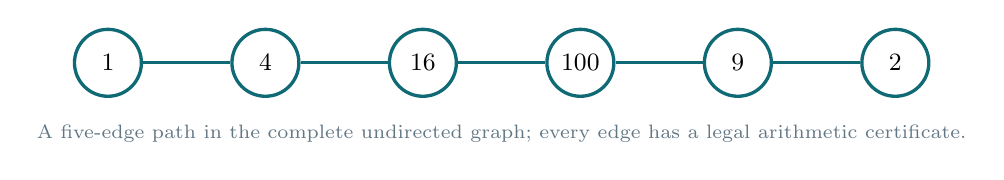
\begin{tikzpicture}[>=Latex, every node/.style={font=\small},x=1cm,y=1cm]
\tikzset{v/.style={circle,draw=tealdark,very thick,fill=white,minimum size=8.5mm,inner sep=0pt},edge/.style={line width=1.1pt,tealdark}}
\foreach \n/\x/\lab in {1/0/1,4/2/4,16/4/16,100/6/100,9/8/9,2/10/2}{\node[v] (n\n) at (\x,0) {\lab};}
\foreach \a/\b in {1/4,4/16,16/100,100/9,9/2}{\draw[edge] (n\a)--(n\b);}
\node[font=\scriptsize,color=slate] at (5,-.9) {A five-edge path in the complete undirected graph; every edge has a legal arithmetic certificate.};
\end{tikzpicture}
\caption{Explicit route proving $d_G(1,2)\le5$. Its integer multiples prove the uniform doubling upper bound. The disjoint radius-two balls in Equation~\eqref{eq:balls} prove sharpness.}
\label{fig:doubling}
\end{figure}

\subsection{Why the other sharp constants need their own certificates}
The scaling method proves the doubling upper bound because the pair $(n,2n)$ is a scalar multiple of $(1,2)$. It does not prove the successor or consecutive-square bounds, because $(n,n+1)$ and $(n^2,(n+1)^2)$ do not form one scaling orbit. Geometry v1.4 establishes $\sup d(n,n+1)=6$ using nine parametric path families and gives a sharpness certificate at $(163,164)$. It establishes $\sup d(n^2,(n+1)^2)=5$ using a separate finite family of polynomial path identities and a sharpness certificate at $(23^2,24^2)$ \cite{geometry}. We rely on those proofs rather than substituting finite-window numerical agreement for global sharpness.

\subsection{A consequence: logarithmic reachability}
The source geometry theorem also yields
\begin{equation}\label{eq:logdistance}
d_G(1,n)\le 11\lfloor\log_2n\rfloor\quad(n\ge2).
\end{equation}
The argument reads the binary digits of $n$, using doubling paths of length at most $5$ and successor paths of length at most $6$. This is a genuine statement about the entire infinite graph: the distance from $1$ is controlled logarithmically in integer magnitude. It does not mean that the induced finite graph on $\{1,\ldots,n\}$ contains the same short routes; routes in the full graph can leave that finite window.

\section{A taxonomy of invariants}
\label{sec:invariants}
The expression ``an invariant of the substrate'' has meaning only after the object, the allowed equivalences, and the relevant auxiliary structures have been specified. The three sharp distances are no less exact for depending on integer labels; they belong to a different invariant category than girth.

\begin{definition}[Abstract graph invariant]
A quantity $I(G)$ is an \emph{abstract graph invariant} if $I(G)=I(H)$ whenever $G\iso H$ as unlabelled graphs. Girth, connectedness, the degree multiset (where meaningful), and a finite graph's cycle rank are examples. The nonbacktracking spectrum of a finite graph, defined by its directed-edge transition matrix, is also preserved by graph isomorphism.
\end{definition}

\begin{definition}[Arithmetic-labelled graph invariant]
Let $\G$ denote the graph $G$ together with its distinguished identification $V(G)=\N$ and the arithmetic relations on its vertices. An \emph{arithmetic-labelled metric invariant} may use $d_G$ together with specified number-theoretic pairings. For example,
\begin{equation}\label{eq:arithmeticI}
I_{+1}(\G)=\sup_{n\ge1}d_G(n,n+1),\quad
I_{\times2}(\G)=\sup_{n\ge1}d_G(n,2n),\quad
I_{\square}(\G)=\sup_{n\ge1}d_G(n^2,(n+1)^2).
\end{equation}
These quantities are preserved under isomorphisms of the enriched structure that respect the corresponding arithmetic relations, but are not claimed to be invariant under an arbitrary graph isomorphism that scrambles the integer names.
\end{definition}

An integer label can always be forgotten to obtain an abstract graph. Forgetting can destroy the ability to ask questions such as ``how far apart are consecutive integers?'' There is no mathematical defect in requiring arithmetic labels; one simply has to state the correct category of the theorem.

\begin{definition}[Graph-history invariant]
For a finite undirected graph $F$, let $\vec E(F)$ denote its directed edges and define the \emph{nonbacktracking matrix}
\begin{equation}\label{eq:BF}
B_F(e,f)=\begin{cases}
1,&\operatorname{head}(e)=\operatorname{tail}(f)\text{ and }f\ne\bar e,\\
0,&\text{otherwise}.
\end{cases}
\end{equation}
Its nonbacktracking entropy is $h_{\NB}(F)=\log\rho(B_F)$ when $\rho(B_F)>0$, with standard conventions for acyclic finite graphs. The construction $F\mapsto B_F$ and its spectral invariants are determined by $F$ and the uniform no-immediate-reversal rule.
\end{definition}

\begin{definition}[Selected-system invariant]
Let $\sigma$ be a legal autonomous selector on positive integers $x\ge2$, with $\sigma(x)\in\N$ and $\sigma(x)\mid x$ (so branch $N=1$ is permitted). Define
\begin{equation}\label{eq:Fsigma}
F_\sigma(x)=T_{\sigma(x)}(x).
\end{equation}
A \emph{selected-system invariant} is a quantity associated to the resulting forward map, its selected orbit, or its itinerary $\bigl(\sigma(x_t)\bigr)_{t\ge0}$. It depends, in general, on $\sigma$, the set of admissible starts, and the observable used to encode the orbit. Prime-fire selectors such as MAXPP form the narrower subclass whose admissible branch labels are primes (and hence at least $2$); the always-legal selector $\sigma_1\equiv1$ of Section~\ref{sec:selection} is in the broader class.
\end{definition}

\begin{table}[htbp]
\centering\small
\caption{Four levels of invariance. ``Intrinsic'' always refers to a declared object and construction.}
\label{tab:tax}
\begin{tabularx}{\textwidth}{@{}p{29mm}X X@{}}
\toprule
\textbf{Level} & \textbf{Examples} & \textbf{Dependence and equivalence}\\
\midrule
Abstract graph & Connectivity, girth, local degrees, cycle rank of a finite subgraph & Preserved by graph isomorphism; independent of trajectory selection.\\
Arithmetic-labelled graph & $I_{+1}=6$, $I_{\times2}=5$, $I_{\square}=5$ & Uses the arithmetic relations between designated vertices; preserved by enriched-graph equivalences.\\
Graph-history & $h_{\NB}(F)$, nonbacktracking spectrum, periodic-history counts, $H_{\mathrm{fin}}(G)$ & Uses the graph and a fixed admissibility rule for histories, not a branch-priority selector.\\
Autonomous selection & MAXPP $\theta$, its growth $\gamma$, ADJ4 return gain and residue law & Requires an additional selector $\sigma$, a branch alphabet/ordering, and sometimes a designated section or initial seed.\\
\bottomrule
\end{tabularx}
\end{table}

\subsection{Can an invariant be intrinsic and still depend on a convention?}
Yes. The choice to make all legal edges undirected is a \emph{construction convention}. Once specified, the graph's invariants are intrinsic \emph{to that graph}. Similarly, a nonbacktracking shift has an explicit history convention; its entropy is intrinsic to the finite graph with this specified, uniform path rule. A rule prescribing a priority between competing arithmetic branches is a different construction: it selects a path, and its dynamical constants belong to that selected system.

The distinction is not between ``chosen'' and ``unchosen'' mathematics in an absolute sense. All mathematical objects are defined by choices of axioms and conventions. The distinction is between \emph{global properties of a fully specified all-branch object} and \emph{properties of an additional path-selection mechanism}.

\begin{scopebox}
\textbf{A useful negative test.} If a claimed constant changes when the selector is altered but the transition law and all-branch graph are held fixed, it is not an intrinsic invariant of the all-branch graph. If it can be derived and verified from the edge relation without mentioning a selector, it belongs to the geometric or graph-history layer. This test identifies provenance; it does not by itself establish mathematical novelty.
\end{scopebox}

\subsection{Structure, representation and selection: a projection principle}
\label{sec:projection}
The hierarchy so far separates the arithmetic structure from a selected trajectory. When a mathematical structure is visualized, a third object enters: its representation. Mathematics offers a clean precedent. The $240$ roots of the $E_8$ root system have squared length $2$ in $\mathbb R^8$ and split as $112$ integer roots and $128$ half-integer roots. Joining two roots when their inner product equals $1$ gives a graph in which every root has $56$ neighbours, so $6720$ edges \cite{conwaysloane,humphreys}. These relations are fixed in eight dimensions. The familiar planar image of $E_8$ is a projection of that configuration; it displays a pattern, but it does not create the adjacency it shows.

The comparison is methodological only. $E_8$ is finite, regular of degree $56$ and has a large symmetry group, whereas $G$ is infinite, has degrees $\tau(x)+\#\{q\ge2:q^2\mid x\}$ and is not vertex-transitive (Corollary~\ref{cor:nonhom}). No lattice, root-system or Lie-theoretic structure is claimed for $G$. Figure~\ref{fig:e8view} reproduces the supplied planar $E_8$ image as an explicit illustration of the distinction between an object and its view. The UNNS plot in the same figure and the shortcut witness in Figure~\ref{fig:collision} provide arithmetic examples, without identifying their geometry with $E_8$.

\begin{figure}[!htbp]
\centering
\begin{minipage}[t]{.45\textwidth}
  \vspace{0pt}\centering
  \fcolorbox{ltline}{black}{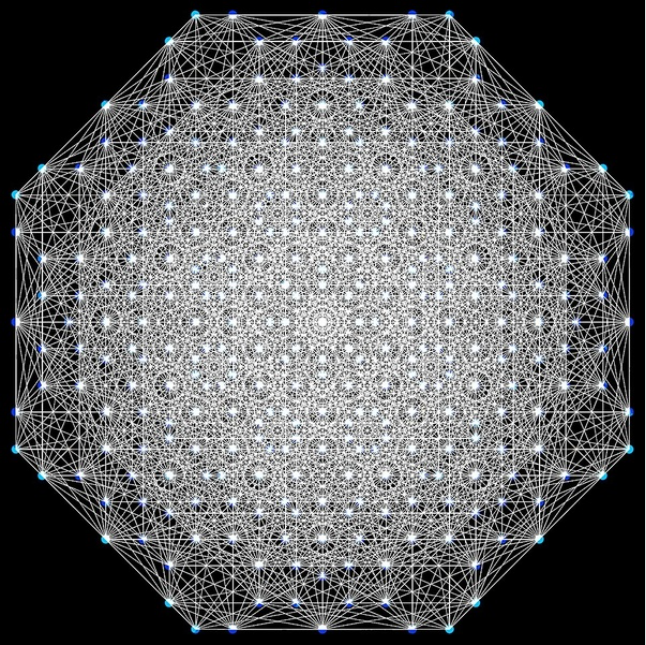
\includegraphics[width=.94\linewidth]{e8_projection_misaki_ohta_crop.png}}\\[2pt]
  {\small\bfseries Eight-dimensional root configuration}\\[-1pt]
  {\footnotesize Planar projection (illustration, not coordinate data)}
\end{minipage}\hfill
\begin{minipage}[t]{.49\textwidth}
  \vspace{0pt}\centering
  {\small\bfseries Exact two-coordinate UNNS projection}\\[1pt]
  {\footnotesize $P=\{2,3\}$; horizontal $v_2$, vertical $v_3$}\\[5pt]
  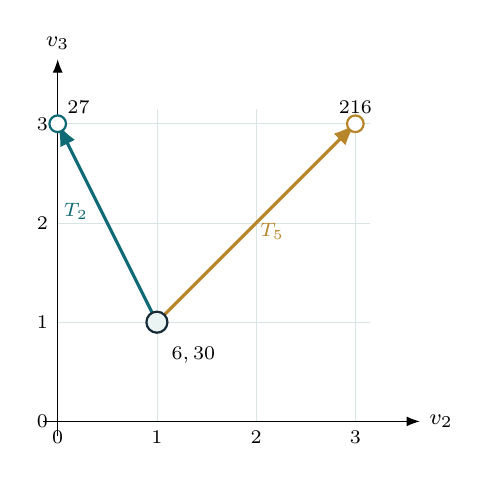
\begin{tikzpicture}[x=1.26cm,y=1.26cm,>=Latex,font=\footnotesize]
   \draw[step=1.26cm,ltline!70,very thin] (0,0) grid (3.15,3.15);
   \draw[->,thin] (-.15,0)--(3.65,0) node[right] {$v_2$};
   \draw[->,thin] (0,-.15)--(0,3.65) node[above] {$v_3$};
   \foreach \a in {0,1,2,3}{\node[below] at (\a,0){\scriptsize\a};\node[left] at (0,\a){\scriptsize\a};}
   \coordinate (start) at (1,1);
   \coordinate (dsttwo) at (0,3);
   \coordinate (dstfive) at (3,3);
   \draw[->,line width=1.1pt,color=tealdark] (start)--(dsttwo) node[pos=.56,left=1pt] {\scriptsize $T_2$};
   \draw[->,line width=1.1pt,color=ochre] (start)--(dstfive) node[pos=.58,below=2pt] {\scriptsize $T_5$};
   \filldraw[fill=white,draw=tealdark,thick] (dsttwo) circle (3pt);
   \filldraw[fill=white,draw=ochre,thick] (dstfive) circle (3pt);
   \filldraw[fill=pale,draw=ink,thick] (start) circle (3.8pt);
   \node[above right] at (dsttwo) {\scriptsize $27$};
   \node[above] at (dstfive) {\scriptsize $216$};
   \node[below right,align=left] at (1.05,.85) {\scriptsize $6,30$};
  \end{tikzpicture}\\[3pt]
  {\footnotesize $T_2(6)=27$,\quad $T_5(30)=216$}\\
  {\footnotesize $\pi_P(6)=\pi_P(30)=(1,1)$}
\end{minipage}
\caption{Two different uses of projection. \emph{Left:} the familiar two-dimensional view of a fixed eight-dimensional $E_8$ root configuration (image: \emph{A two-dimensional projection of the shortest vectors of an $E_8$ lattice}, by Misaki Ohta, licensed under \href{https://creativecommons.org/licenses/by-sa/4.0/}{CC BY-SA 4.0}; cropped to remove the web caption, otherwise unmodified). \emph{Right:} an exact two-coordinate visualization of separately verified UNNS steps; the two start states $6$ and $30$ share one plotted point, but $T_5$ is legal only from $30$. The right-hand plot does not display the complete infinite graph.}
\label{fig:e8view}
\end{figure}

\paragraph{Prime-valuation coordinates.} By Theorem~\ref{thm:valuation} every legal step is a translation of the exponent vector, $\vv(T_N(x))=\vv(x)+\boldsymbol\tau_N$, so $G$ already has an exact representation in the space of finitely supported exponent vectors. Unlike $E_8$, this space has no fixed dimension. For a finite set $P$ of primes put $\pi_P(x)=\bigl(v_p(x)\bigr)_{p\in P}$, and write $\pi_P(\boldsymbol\tau_N)$ for the restriction of $\boldsymbol\tau_N$ to the coordinates in $P$. Then
\begin{equation}\label{eq:projtrans}
\pi_P\bigl(T_N(x)\bigr)=\pi_P(x)+\pi_P(\boldsymbol\tau_N).
\end{equation}
For example $T_2(6)=27$ reads $(1,1,0)\mapsto(0,3,0)$ in the primes $\{2,3,5\}$, a genuine translation.

\begin{definition}[Projected graph]
The \emph{projected graph} $\pi_P(G)$ has vertex set $\pi_P(\N)\subset\mathbb Z_{\ge0}^{|P|}$, and distinct points $u,w$ are adjacent exactly when some edge $\{a,b\}\in E(G)$ has $\pi_P(a)=u$ and $\pi_P(b)=w$.
\end{definition}

\begin{proposition}[Projection is nonexpanding]\label{prop:nonexpanding}
For all $a,b\in\N$, $\;d_{\pi_P(G)}\bigl(\pi_P(a),\pi_P(b)\bigr)\le d_G(a,b)$.
\end{proposition}
\begin{proof}
Map a shortest path $a=x_0,\dots,x_k=b$ in $G$ to $\pi_P(x_0),\dots,\pi_P(x_k)$. Consecutive terms are equal or adjacent in $\pi_P(G)$ by definition; deleting repetitions leaves a walk of length at most $k$.
\end{proof}

\begin{proposition}[Legality preservation under finite prime projections]\label{prop:legality}
Let $P$ be a finite set of primes and $N\ge1$. The following are equivalent.
\begin{enumerate}[label=(\alph*)]
\item Whenever $\pi_P(x)=\pi_P(x')$, we have $N\mid x\iff N\mid x'$.
\item Every prime divisor of $N$ lies in $P$.
\end{enumerate}
In particular, for every finite $P$ and every prime $q\notin P$, the legality of $T_q$ is not a function of $\pi_P(x)$.
\end{proposition}
\begin{proof}
(b)$\Rightarrow$(a): by Theorem~\ref{thm:valuation}, $T_N$ is legal at $x$ exactly when $v_p(x)\ge v_p(N)$ for all primes $p$. For $p\notin P$ we have $v_p(N)=0$, so only the coordinates $p\in P$ matter, and these are given by $\pi_P(x)$.
(a)$\Rightarrow$(b): suppose a prime $q\notin P$ divides $N$. Take $x=N$ and $x'=N/q$. They agree in every coordinate $p\ne q$, hence $\pi_P(x)=\pi_P(x')$, but $N\mid x$ and $N\nmid x'$.
\end{proof}

\begin{observation}[Two collisions]\label{obs:collisions}
Take $P=\{2,3\}$. First, $\pi_P(6)=\pi_P(30)=(1,1)$, yet $T_5$ is legal at $30$ and illegal at $6$. Second, as illustrated in Figure~\ref{fig:collision}, $\pi_P(1)=\pi_P(5)=(0,0)$, so the edges $\{1,4\}$ and $\{5,36\}$ project to $(0,0)\!-\!(2,0)$ and $(0,0)\!-\!(2,2)$. Hence $d_{\pi_P(G)}\bigl((2,0),(2,2)\bigr)\le2$, whereas $d_G(4,36)\ge3$: indeed $4\not\sim36$, and $N_G(4)=\{1,16,18,25\}$ is disjoint from $N_G(36)=\{5,8,9,144,162,192,225,294,400,507,722,1369\}$.
\end{observation}

\begin{figure}[!htbp]
\centering
\begin{minipage}[c]{.45\textwidth}
 \centering
 {\bfseries Original arithmetic vertices}\\[5pt]
 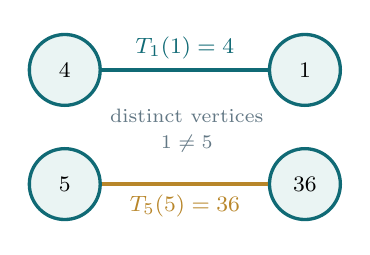
\begin{tikzpicture}[x=1cm,y=1cm,font=\footnotesize]
   \tikzset{v/.style={draw=tealdark,fill=pale,very thick,circle,minimum size=9mm,inner sep=0pt}}
   \node[v] (a) at (.4,1.45) {$4$};
   \node[v] (b) at (3.45,1.45) {$1$};
   \node[v] (c) at (.4,0) {$5$};
   \node[v] (d) at (3.45,0) {$36$};
   \draw[line width=1.2pt,tealdark] (b)--node[above] {$T_1(1)=4$} (a);
   \draw[line width=1.2pt,ochre] (c)--node[below] {$T_5(5)=36$} (d);
   \node[align=center,text=slate] at (1.95,.68) {\scriptsize distinct vertices\\\scriptsize $1\ne5$};
 \end{tikzpicture}\\[3pt]
 {\footnotesize $N_G(4)\cap N_G(36)=\varnothing$}\\[-1pt]
 {\footnotesize hence $d_G(4,36)\geq 3$}
\end{minipage}\hfill
\begin{minipage}[c]{.52\textwidth}
 \centering
 {\bfseries Projected graph $\pi_{\{2,3\}}(G)$}\\[5pt]
 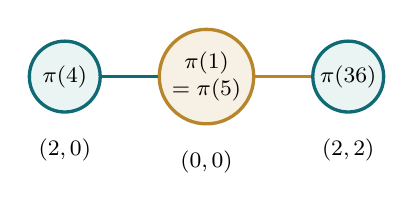
\begin{tikzpicture}[x=1cm,y=1cm,font=\footnotesize]
   \tikzset{q/.style={draw=tealdark,fill=pale,very thick,circle,minimum size=9mm,inner sep=0pt}}
   \node[q] (a) at (.4,.85) {$\pi(4)$};
   \node[q,draw=ochre,fill=ochre!12,minimum size=12mm,align=center] (b) at (2.2,.85) {$\pi(1)$\\$=\pi(5)$};
   \node[q] (c) at (4.0,.85) {$\pi(36)$};
   \draw[line width=1.2pt,tealdark] (a)--(b);
   \draw[line width=1.2pt,ochre] (b)--(c);
   \node[below=2mm of a] {$(2,0)$};
   \node[below=2mm of b] {$(0,0)$};
   \node[below=2mm of c] {$(2,2)$};
 \end{tikzpicture}\\[3pt]
 {\footnotesize $d_{\pi_P(G)}((2,0),(2,2))\leq 2$}
\end{minipage}
\caption{A rigorously certified projection-created shortcut. Only two genuine source edges are drawn at left; the labels $1$ and $5$ are \emph{not} identified in $G$. Under $P=\{2,3\}$ they collapse to the same projected vertex $(0,0)$, creating the displayed two-edge path between $\pi_P(4)$ and $\pi_P(36)$. The full-graph neighborhood calculation in Observation~\ref{obs:collisions} proves that the unprojected endpoints have distance at least three. The diagram is a finite witness, not a claim that these are the only edges of either entire graph.}
\label{fig:collision}
\end{figure}

\paragraph{Projection versus selection.} A projection acts on \emph{states}: it forgets coordinates, can merge distinct vertices, and by Proposition~\ref{prop:nonexpanding} can only shorten distances. A selector acts on the \emph{relation}: it chooses one legal outgoing branch at each state. Neither changes $E(G)$. They are different operations, and a projection can be faithful for a selected system without being faithful for the structure: Section~\ref{sec:primefire} shows that after finitely many high-prime firings a prime-fire orbit is carried by the translations \eqref{eq:two-vectors} in $(v_2,v_3)$, but this is a statement about that orbit and says nothing about legality across $G$.

\begin{table}[htbp]
\centering\small
\caption{Structure, representation and selection.}
\label{tab:three}
\begin{tabularx}{\textwidth}{@{}p{24mm}p{20mm}X X@{}}
\toprule
\textbf{Layer} & \textbf{Object} & \textbf{Operation} & \textbf{Effect on the structure}\\
\midrule
Structure & $\A,\ G$ & All legal transitions and all legal edges & Fixed once the law and the edge convention are declared.\\
Representation & $\pi_P(G)$ & Coordinate map on states & Merges states, hides legality, can shorten distances; $G$ unchanged.\\
Selection & $F_\sigma$ & One legal branch $\sigma(x)$ per state & Picks directed edges for an orbit; $E(G)$ unchanged.\\
\bottomrule
\end{tabularx}
\end{table}

\begin{takeaway}
\textbf{Reading rule.} Adjacency, distance, cycle structure and history entropy are determined in $G$. A projection may be used to draw $G$, but a quantity read off $\pi_P(G)$ is a property of $G$ only when a preservation theorem says so. Apparent symmetries, clusters or short routes in a picture are representation-dependent until then.
\end{takeaway}


\section{Intrinsic histories, book graphs, and spectral entropy}
\label{sec:entropy}
The all-branch graph contains more information than distances between vertices. It also contains the collection of all finite walks and, under a standard prohibition on immediately traversing the preceding edge backward, the collection of nonbacktracking histories. This is a graph-derived symbolic system, not a deterministic selector operating the arithmetic rule forward.

\subsection{The arithmetic book graphs}
For each integer $x\ge2$, let $D(x)=\{N\mid x:N\ge2\}$, and write
\begin{equation}\label{eq:bookdefs}
y_N=\frac{x(N+1)^2}{N},\qquad b=|D(x)|=\tau(x)-1.
\end{equation}
The finite graph $F(x)$ consists of the hub vertices $x,4x$, the interior vertices $y_N,4y_N$ for $N\in D(x)$, and the edges
\begin{equation}\label{eq:bookedges}
\{x,4x\},\qquad\{x,y_N\},\qquad\{y_N,4y_N\},\qquad\{4y_N,4x\}.
\end{equation}
All edges are legal edges of $G$: the first and middle ``scaling'' edges use $N=1$, while the other two use the branch $N$ and its scaling by $4$. The parameter $N$ is allowed precisely because $N\mid x$. The source Graph Entropy manuscript proves the book structure and, for $F_m=F(2^m)$, that $F_m$ is induced on its own vertex set \cite{entropy}. For general $x$ we prove interior-vertex distinctness below. The explicitly specified edge set defines $F(x)$ as a subgraph of $G$; the argument does not require a claim that every general $F(x)$ is induced.

\begin{proposition}[Book structure and cycle rank; derived from the construction]\label{prop:bookrank}
For $x\ge2$ and $b=\tau(x)-1$, the graph $F(x)$ is a theta graph with one path of length $1$ and $b$ internally disjoint paths of length $3$ between the same two hubs. In particular,
\begin{equation}\label{eq:bookcount}
|V(F(x))|=2b+2,\qquad |E(F(x))|=3b+1,\qquad
\beta_1(F(x))=b.
\end{equation}
\end{proposition}
\begin{proof}
For each $N\in D(x)$, the three-edge path $x-y_N-4y_N-4x$ has two interior vertices. These vertices are distinct for every $x\ge2$, as follows. Recall that $r_N=(N+1)^2/N$ is strictly increasing and $y_N=x\,r_N$. Therefore the $y_N$ are pairwise distinct, as are the $4y_N$. All are strictly greater than $4x$, since $r_N\ge 9/2$ for $N\ge2$, so none is a hub.

It remains to exclude a cross-family equality $y_N=4y_M$, which would give $r_N=4r_M$. Put $d=\gcd(M,4)\in\{1,2,4\}$. Because $r_N=(N+1)^2/N$ and $4r_M=4(M+1)^2/M$ are each written with coprime numerator and denominator after reduction, equality forces
\[
N=\frac{M}{d},\qquad (N+1)^2=\frac4d\,(M+1)^2 .
\]
If $d=1$, then $N=M$ yet $N+1=2(M+1)$, which is impossible. If $d=2$, a positive integer square would equal twice another positive integer square, which is impossible. If $d=4$, the equality of squares gives $N=M$ while the denominator gives $N=M/4$, again impossible. Hence no cross-family equality exists.

There is also the direct hub edge $x-4x$. The graph $F(x)$ therefore has $2+2b$ vertices and $1+3b$ edges and is precisely a theta graph with $b$ internally disjoint three-edge pages and one direct edge. Its cycle rank is $|E|-|V|+1=b$.
\end{proof}

\begin{figure}[htbp]
\centering
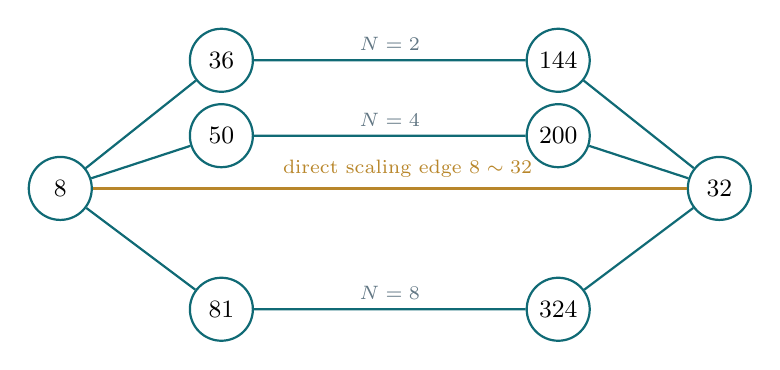
\begin{tikzpicture}[>=Latex,scale=.93,every node/.style={font=\small},v/.style={circle,draw=tealdark,thick,fill=white,minimum size=8mm,inner sep=0pt}]
\node[v] (u) at (0,0) {$8$};\node[v] (v) at (9,0) {$32$};
\draw[ochre,very thick] (u) -- (v) node[pos=.53,above,font=\scriptsize,color=ochre] {direct scaling edge $8\sim32$};
\foreach \y/\aa/\bb/\lab in {1.75/36/144/{N=2},.72/50/200/{N=4},-1.65/81/324/{N=8}}{
 \node[v] (a\aa) at (2.2,\y) {$\aa$}; \node[v] (b\bb) at (6.8,\y) {$\bb$};
 \draw[tealdark,thick] (u)--(a\aa)--(b\bb)--(v);
 \node[font=\scriptsize,color=slate] at (4.5,\y+.22) {$\lab$};
}
\end{tikzpicture}
\caption{The explicit arithmetic book $F(8)=F_3$. The hubs $8$ and $32$ have one direct edge and three disjoint length-three alternatives. The numbers and edges are obtained by legal arithmetic transitions.}
\label{fig:book}
\end{figure}

\subsection{The exact spectral law}
The nonbacktracking entropy of these books is computed from a single algebraic equation. This is a theorem about the constructed finite graph and its full history space, rather than about a selector following a preferred branch.

\begin{theorem}[Exact book-graph entropy; source theorem]\label{thm:bookentropy}
For $m\ge1$ there is a unique positive real root $\lambda_m$ of
\begin{equation}\label{eq:cubic}
\lambda_m^3-\lambda_m^2+\lambda_m=m,
\end{equation}
and
\begin{equation}\label{eq:entropy}
h_{\NB}(F_m)=\log\lambda_m.
\end{equation}
For $m\ge2$ the same theorem gives
\begin{equation}\label{eq:entropybound}
\frac13\log m<h_{\NB}(F_m)<\frac13\log m+\frac{1}{3m^{1/3}}.
\end{equation}
\end{theorem}
\begin{proof}[Explanation of the defining equation]
The theta-graph transfer calculation in Theorem 5.1 of \cite{entropy} gives the Perron-root equation
\[
\frac{1}{\lambda+1}+\frac{m}{\lambda^3+1}=1
\]
for a theta graph with one path of length $1$ and $m$ paths of length $3$. Rearranging,
\[
m=\frac{\lambda(\lambda^3+1)}{\lambda+1}
  =\lambda(\lambda^2-\lambda+1)
  =\lambda^3-\lambda^2+\lambda.
\]
The unique root $\lambda\ge1$ is the nonbacktracking spectral radius, so the entropy is $\log\lambda$. The bounds in \eqref{eq:entropybound} are established in Lemma 6.2 and Theorem 6.3 of \cite{entropy}; they follow from bracketing $\lambda_m$ between $m^{1/3}$ and $m^{1/3}+1/3$.
\end{proof}

\subsection{A single arithmetic--topology--entropy correspondence}
Combining Proposition~\ref{prop:bookrank} and Theorem~\ref{thm:bookentropy} yields an exact relationship involving three different kinds of information.
\begin{corollary}[Arithmetic--topology--entropy identity]\label{cor:chain}
For $x\ge2$ and $h=h_{\NB}(F(x))$,
\begin{equation}\label{eq:chain}
\boxed{\tau(x)-1=\beta_1(F(x))=e^{3h}-e^{2h}+e^h.}
\end{equation}
\end{corollary}
\begin{proof}
The first equality is \eqref{eq:bookcount}. By the preceding proof, $F(x)$ is abstractly isomorphic to the $b$-page book $F_b=F(2^b)$ with $b=\tau(x)-1$; its nonbacktracking matrix is therefore the same up to a permutation of directed-edge states. Hence Theorem~\ref{thm:bookentropy} applies to $F(x)$ and not only to the powers-of-two model $F_m$. Substituting $\lambda=e^h$ into \eqref{eq:cubic} with $m=b$ proves the second equality.
\end{proof}

\begin{takeaway}
\textbf{What the equality says.} For this explicitly constructed family---not for arbitrary graphs---the number of divisors of $x$ minus one determines the cycle rank of $F(x)$, which in turn determines its nonbacktracking entropy through an exact cubic equation. It is a correspondence between arithmetic-labelled construction, graph topology, and graph-history dynamics.
\end{takeaway}

\subsection{A worked exact example}
Take $x=64=2^6$. Then $\tau(64)=7$, so $b=6$, $F(64)$ has $14$ vertices, $19$ edges, and $\beta_1=19-14+1=6$. The cubic $\lambda^3-\lambda^2+\lambda=6$ has root $\lambda=2$, yielding
\begin{equation}\label{eq:64}
\boxed{\tau(64)=7,\quad \beta_1(F(64))=6,\quad h_{\NB}(F(64))=\log2.}
\end{equation}
The same entropy occurs for $x=729=3^6$ because its divisor count is also $7$. This equality does not imply the labelled subgraphs $F(64)$ and $F(729)$ are arithmetically identical; rather, their abstract book-graph structures have the same number of pages.

\subsection{Unbounded intrinsic finite-history capacity}
Define
\begin{equation}\label{eq:Hfin}
H_{\mathrm{fin}}(G)=\sup\{h_{\NB}(F):F\subseteq G\text{ is a finite subgraph}\}.
\end{equation}
Since $F_m=F(2^m)$ exists for every $m\ge1$ and its entropy grows as $(1/3)\log m$, the source theorem proves
\begin{equation}\label{eq:unbounded}
H_{\mathrm{fin}}(G)=+\infty.
\end{equation}
More concretely, writing $G[1,X]$ for the subgraph induced on the integer interval $\{1,\ldots,X\}$, the Graph Entropy paper proves a lower bound of the form
\begin{equation}\label{eq:window}
h_{\NB}(G[1,X])\ge\frac13\log\log X-C
\quad\text{for sufficiently large }X,
\end{equation}
with some absolute constant $C$ \cite{entropy}. This is a \emph{lower bound}, not an exact asymptotic formula for the window entropy.

\subsection{Period two and spectral interpretation}
For $m\ge2$, the nonbacktracking matrix of $F_m$ has simple peripheral eigenvalues $+\lambda_m$ and $-\lambda_m$. The associated maximal-entropy Markov chain has period two. Its relative nonperipheral spectral modulus is
\begin{equation}\label{eq:R}
R_m=\sqrt{1-\lambda_m^{-1}+\lambda_m^{-2}}.
\end{equation}
The one-step nonperipheral modulus gap satisfies $1-R_m\sim\tfrac12m^{-1/3}$. The gap relevant to the two-step chain restricted to one parity class is
\begin{equation}\label{eq:two-step}
1-R_m^2=\lambda_m^{-1}-\lambda_m^{-2}\sim m^{-1/3}.
\end{equation}
The two-step gap reaches its maximum at $\lambda_m=2$ (that is, $m=6$) before eventually decreasing toward zero. These qualifications are important: one must not infer ordinary one-step convergence to a unique stationary distribution from a periodic transition matrix.

\section{Autonomous selection: an additional dynamical grammar}
\label{sec:selectors}
The mathematical moment at which a trajectory-selection problem appears is the introduction of an extra rule $\sigma(x)$ specifying which legal branch fires. The selected map $F_\sigma$ is a new object derived from the common transition family. Its orbit and symbolic itinerary can exhibit properties not shared by all selectors.

\subsection{Prime-fire selection and eventual two-dimensionality}\label{sec:primefire}
Restrict the selected branch values to primes. The Prime-Valuation manuscript proves that for every prime-fire selector and every start $x_0\ge2$, only finitely many branches $p\ge5$ are ever fired \cite{prime}. The proof uses the fact that, for a prime $p\ge5$, firing $p$ decreases its own exponent by one while adding only prime factors of $p+1$, all strictly below $p$. A well-founded high-prime potential prevents infinitely many such firings. Once these firings stop, only the active primes $2$ and $3$ remain; higher-prime factors may still be present at constant exponents.

In the coordinates $(\alpha,\beta)=(v_2,v_3)$, the two remaining translations are
\begin{equation}\label{eq:two-vectors}
T_2:(\alpha,\beta)\mapsto(\alpha-1,\beta+2),\qquad
T_3:(\alpha,\beta)\mapsto(\alpha+4,\beta-1).
\end{equation}
The dimensional reduction is itself universal for the stipulated class of prime-fire selectors, but the detailed symbolic dynamics of a particular selector must still be established separately.

\subsection{MAXPP and its irrational rotation}
MAXPP fires the prime whose prime-power part of the current integer is largest. After the high-prime transient, put
\begin{equation}\label{eq:f}
f=\alpha\log2-\beta\log3.
\end{equation}
The two branches shift $f$ by $-\log18$ and $+\log48$, respectively. The reduced dynamics enters an invariant interval of length $\log864$; normalizing gives the irrational rotation number
\begin{equation}\label{eq:theta}
\boxed{\theta_{\mathrm{MAXPP}}=\frac{\log48}{\log864}\approx0.5725296678.}
\end{equation}
The prime-valuation manuscript proves that the eventual branch itinerary is Sturmian for every start $x_0\ge2$:
\begin{equation}\label{eq:sturmian}
p(k)=k+1,\qquad h_{\mathrm{top}}=0,
\end{equation}
and the frequency of branch $2$ is $\theta_{\mathrm{MAXPP}}$ with discrepancy less than one. The growth rate is
\begin{equation}\label{eq:gamma}
\gamma=\theta\log_2\frac92+(1-\theta)\log_2\frac{16}{3}
\approx2.2747033\ \text{bits per step}.
\end{equation}
A sharpened post-entry estimate, written relative to the state $x_T$ at entrance into the rotation regime, is
\begin{equation}\label{eq:deviation}
\left|\log_2\frac{x_{T+n}}{x_T}-\gamma n\right|
<\log_2\frac{32}{27},\qquad n\ge0.
\end{equation}
This is an absolute-value (two-sided) bound on the post-entry residual, not merely a one-sided estimate.
The precise growth estimate and the aperiodic symbolic itinerary coexist: deterministic arithmetic order need not be periodic, and symbolic aperiodicity does not imply positive symbolic entropy.

\subsection{ADJ4 and a certified expanding return}
The ADJ4 manuscript fixes an ordered list of $22$ admissible moves supported on the primes $\{2,3,5,7\}$ and a designated initial state. A legal first-applicable rule generates one autonomous forward trajectory. On a specified return section the selected return has the exact form
\begin{equation}\label{eq:adj}
z' =\frac{2869z+\delta_{a,r}}{49},\qquad r=z\bmod49,
\end{equation}
where the finite correction table $\delta_{a,r}$ is established by a computer-assisted exact certificate \cite{adj}. The leading factor
\begin{equation}\label{eq:adjfactor}
\boxed{\frac{2869}{49}=\frac{151}{49}\cdot\frac{38}{2}\cdot\frac{2}{2}}
\end{equation}
is derived from three exponent-transfer regimes: a period-$45$ rotation-like block, a period-$11$ register cycle, and a variable-length branch-$4$ run. The manuscript's non-eventual-periodicity theorem concerns the branch itinerary, not the trivially increasing integer states. Its proof uses the complete return mechanism, including the certified residue corrections; a leading multiplier exceeding one is not, by itself, sufficient to prove the symbolic statement.

\subsection{An elementary selector contrast on one fixed graph}\label{sec:selection}
The selector dependence can be demonstrated without a complicated construction. Under the general legal-selector definition above, define the always-legal selector $\sigma_1(x)=1$ for all positive integers $x$. Its selected orbit is
\begin{equation}\label{eq:trivialselector}
x_t=4^t x_0,\qquad \sigma_1(x_t)=1\quad\text{for every }t.
\end{equation}
Its branch itinerary is constant and its binary-logarithmic growth rate is exactly $2$ bits per step. On the very same ambient transition family and graph $G$, the MAXPP selector (restricted to prime branches) gives the Sturmian itinerary and the distinct growth constant \eqref{eq:gamma}. Thus the complete unselected graph is unchanged while the selected symbolic regime changes dramatically. This example does not claim that every finite branch restriction can be handled by the same proof; it isolates the logical dependence on a declared selector.

\subsection{These constants are not graph invariants}
Changing the selector can change branch frequencies, selected growth laws, return maps, periodicity properties, and symbolic complexity while leaving $G$ unchanged. Thus $\theta_{\mathrm{MAXPP}}$, $\gamma_{\mathrm{MAXPP}}$, and $2869/49$ are invariants of the \emph{specified selected systems} under an appropriate notion of dynamical equivalence. They are not intrinsic constants of the undirected all-branch graph.

\begin{table}[htbp]
\centering\small
\caption{Four source manuscripts reclassified by object and mathematical role.}
\label{tab:papers}
\begin{tabularx}{\textwidth}{@{}p{31mm}p{34mm}X@{}}
\toprule
\textbf{Manuscript} & \textbf{Object studied} & \textbf{Principal result families}\\
\midrule
Geometry v1.4 & All-branch graph $G$ with integer labels & Connectedness, degree, scaling, sharp arithmetic distances $(6,5,5)$; cycle results with U3 (odd girth $5$) and U3-COR (girth $4$).\\
Graph Entropy v1.5 & $G$, finite books $F(x)$, nonbacktracking histories & Exact cubic entropy, spectral and periodic-history laws, unbounded finite-history capacity, arithmetic--topology identity.\\
Prime-Valuation v1.2 & Prime-fire maps; MAXPP and other selected systems & High-prime reduction, irrational rotation, Sturmian itinerary, growth, support renewal, guard complexity.\\
Aperiodicity v2.7 & ADJ4 priority-selected forward orbit & Three-regime exponent exchange, certified return $2869/49$, non-eventually-periodic branch itinerary.\\
\bottomrule
\end{tabularx}
\end{table}


\section{Intrinsic structure versus selected dynamics: the formal separation}
\label{sec:separation}
We can now state the hierarchy without relying on metaphors about ``worlds'' or ``handcrafted trajectories.'' The following is a formal classification of the cited mathematical objects and the dependencies of their claims.

\begin{proposition}[Intrinsic--selected separation; derived classification]\label{prop:separation}
Let $\A$ be the transition system \eqref{eq:A}, and let $G$ be \eqref{eq:G}.
\begin{enumerate}[label=(\roman*)]
\item Every invariant defined solely from $G$ is independent of the choice of a forward selector $\sigma$.
\item Every quantity defined from $(G,\text{integer arithmetic relations})$, including \eqref{eq:arithmeticI}, is independent of $\sigma$, but may depend on the retained arithmetic labelling.
\item For any finite subgraph $F\subseteq G$, the nonbacktracking shift and its finite-state spectral invariants are determined by $F$ and the fixed nonbacktracking convention; their definition contains no branch-priority rule.
\item A quantity defined from a selected map $F_\sigma$ or its itinerary is in general dependent on $\sigma$ and is not, merely for that reason, an invariant of $G$.
\end{enumerate}
\end{proposition}
\begin{proof}
Assertions (i) and (ii) follow from Proposition~\ref{prop:selectorfree}, with the second carrying the additional arithmetic relations as fixed data. For (iii), the entries of $B_F$ are uniquely determined by adjacency of directed edges and the exclusion $f\ne\bar e$; there is no input from $\sigma$. Assertion (iv) is immediate from the definition $F_\sigma(x)=T_{\sigma(x)}(x)$, which changes when the selector changes. No assertion is made that every possible invariant \emph{must} change for some choice of selector; only that selector independence is not automatic.
\end{proof}

The proposition names an organizational distinction whose constituent facts are straightforward. It should not be misreported as a new difficult theorem about the dynamics. Its value is to make the quantifiers and the mathematical objects explicit.

\subsection{Which choices occur at which stage?}
\begin{table}[htbp]
\centering\small
\caption{Audit of mathematical choices, from the founding transformation to specific dynamical regimes.}
\label{tab:choices}
\begin{tabularx}{\textwidth}{@{}p{29mm}X X@{}}
\toprule
\textbf{Stage} & \textbf{Specified data} & \textbf{What is not yet chosen}\\
\midrule
Transition law & Formula $T_N$, positive-integer domain, legality $N\mid x$, admissible branch labels & No branch priority and no orbit.\\
All-branch graph & Every legal edge, symmetry of traversal, unit edge lengths & No next-edge selector and no preferred geodesic.\\
Geometric theorem & Pairs of vertices or arithmetic families, e.g. $(n,2n)$ & No trajectory used in the \emph{definition} of $d_G$. A proof may exhibit paths as certificates.\\
History shift & Directed edges of $F$, prohibition of immediate reversal & No designated infinite history and no priority among continuations.\\
Autonomous forward map & State-only selector $\sigma$, tie handling, branch restrictions & A particular seed is optional unless the theorem addresses a chosen orbit.\\
Return theorem & Selector, section, return criterion, parameters, sometimes seed & None of these is forced merely by knowing $G$.\\
\bottomrule
\end{tabularx}
\end{table}

\subsection{Why an explicit proof path is not an engineered dynamical trajectory}
To prove a graph-distance upper bound, one is allowed to \emph{exhibit a path} in the already defined graph. Choosing such a path is an act of mathematical proof search. It does not alter the edge relation, and it does not define how a dynamical state chooses its next branch. Similarly, a shortest-path argument quantifies over all paths whether or not a proof displays any particular path.

The route $1\sim4\sim16\sim100\sim9\sim2$ provides an existence certificate: $d_G(1,2)\le5$. The separate disjoint-ball argument supplies a universal obstruction to shorter paths. Together they establish an intrinsic metric fact. Neither construction modifies $G$ or prescribes a selector that must follow the displayed route in subsequent evolution.

This is the most direct response to the criticism that the graph's geometry was \emph{made} to display its distance constants by selecting special histories. The definitions and the proof do not do that. A different criticism---whether the original rule and its conventions are mathematically interesting or uniquely motivated---is legitimate and should be answered by independent comparison, robustness, and theorem strength, not by treating graph paths as selected trajectories.

\subsection{The boundary of the intrinsic claim}
Several qualifications are necessary for precision:
\begin{enumerate}
\item \textbf{Dependence on the arithmetic rule.} A different family of rational multipliers or different legality domains can produce a different graph and different invariants. No universal stability across arbitrary rule changes is claimed.
\item \textbf{Dependence on edge conventions.} Turning forward arrows into undirected unit edges is part of the graph definition. If directed distance or weighted distance is used instead, the results must be reformulated.
\item \textbf{Dependence on vertex labelling.} The distance triple uses integer successor, doubling and consecutive-square relations. These are part of the arithmetic enrichment of $G$.
\item \textbf{Dependence on history conventions.} Positive nonbacktracking entropy is not the entropy of strictly forward integer trajectories. It belongs to a graph history system that permits inverse graph traversal and excludes immediate reversal.
\item \textbf{Dependence of ADJ4 on certification.} Its exact leading multiplier is transparent from exponent transfers, but its full finite return table and global itinerary theorem invoke an exact computer-assisted proof.
\end{enumerate}

These boundaries are features of an accurate mathematical classification, not concessions that invalidate the established proofs.

\section{Relation to established theories}
\label{sec:comparisons}
A useful scientific comparison concerns \emph{architecture} rather than identity. A base structure is defined; one studies its intrinsic invariants; then one constructs additional dynamical systems on it. The UNNS hierarchy resembles several familiar patterns, with important differences.

\subsection{Cayley graphs and word metrics}
A group $\Gamma$ together with a generating set $S$ determines its Cayley graph and word metric. Geometry is then studied independently of any particular random walk on $\Gamma$. The analogy to the UNNS construction is the separation between the graph metric and a rule for traversing the graph \cite{loeh}. It is not an equivalence: $G$ is not specified as a Cayley graph, lacks vertex-transitivity, and its nonexpanding scaling maps are not group translations. Moreover, even within geometric group theory, word metrics depend on the chosen generating set; ``intrinsic'' is always relative to fixed structure.

\subsection{Symbolic shifts from directed graphs}
A finite directed graph determines a shift of finite type by permitting consecutive directed edges. Its entropy is the logarithm of the spectral radius of the transition matrix. The nonbacktracking shift fits this classical setting when applied to the directed-edge states of a finite undirected graph. The construction is generic; the arithmetic contribution here is the explicit family of subgraphs $F_m$ and the unusually tractable cubic equation for the Perron root.

\subsection{Ihara--Bass theory}
The nonbacktracking operator and the associated determinant are standard objects in spectral graph theory \cite{kotani,ihara2026}. The Graph Entropy manuscript derives, for the arithmetic book family,
\begin{equation}\label{eq:det}
\det(I-uB_{F_m})=(1-u^6)^{m-1}(1-u^2)
(1-u+u^2-mu^3)(1+u+u^2+mu^3),
\end{equation}
as well as periodic-walk counts and stationary distributions \cite{entropy}. We cite the arithmetic derivation rather than claiming the Ihara--Bass method itself was discovered by the UNNS programme. The distinction is essential for a responsible assessment of mathematical novelty.

\subsection{Sturmian sequences and irrational rotations}
The fact that an irrational rotation can generate a Sturmian word of complexity $p(k)=k+1$ is classical \cite{morse,sturmian}. The specific achievement of MAXPP is that the arithmetic prime-power comparison rule reduces to such a rotation with a concrete logarithmic slope, valid for every nontrivial starting integer after its finite transient. This is an arithmetic realization of an established dynamical regime, with quantitative consequences determined by the arithmetic multipliers.

\subsection{Dynamics on graphs versus graph-defined history spaces}
There is a key difference between a random walk or a deterministic route on $G$ and the nonbacktracking shift of \emph{all} admissible histories. The former adds a transition kernel or a selector; the latter studies the language of possible directed-edge continuations subject to a uniform local rule. Both can be investigated on one graph but need not share entropy, invariant measures, or periodicity classes. The distinction is particularly visible in the UNNS examples: the prime-fire itinerary is Sturmian with zero entropy, while the family of reversible book-graph history systems has unbounded finite-subgraph entropy.

\begin{scopebox}
\textbf{Novelty should be assessed at the right level.} Classical notions such as graph distance, cycle rank, irrational rotation, Sturmian coding, and nonbacktracking spectral radius are established mathematics. The source-specific questions are whether the UNNS arithmetic transition yields new exact identities, sharp bounds, special constructive families, or general principles not immediate from standard templates. The distinction between base objects and secondary dynamics clarifies that assessment; it does not replace it.
\end{scopebox}

\section{A research programme made possible by the hierarchy}
\label{sec:agenda}
The organization developed above suggests tests that can distinguish universal consequences of the fixed arithmetic graph from mechanisms peculiar to selected systems. The following items are \emph{proposed investigations}, not established results.

\subsection{Intrinsic geometry: rigidity and reconstruction}
\textbf{Question G1 (automorphisms).} Determine the automorphism group $\operatorname{Aut}(G)$ of the unlabelled arithmetic graph, or establish strong restrictions on it from local degrees, square-divisibility neighborhoods, and short cycles. Can arithmetic information about certain labels be reconstructed from the abstract graph? If not, which arithmetic relations must be retained to formulate sharp labelled metric laws?

\textbf{Question G2 (higher-power distances).} The sharp values are known for successors and consecutive squares, while a general power-lifting inequality gives $d(n^k,(n+1)^k)\le6k$. Determine sharp suprema for $k\ge3$ or characterize the obstruction to finite universal sharp constants in related families. A positive result would concern the labelled graph and would require no selector.

\textbf{Question G3 (intrinsic metric scaling).} Classify when the nonexpanding scaling inequality $d(ma,mb)\le d(a,b)$ is strict and identify pairs for which equality holds for all $m$. This would expose additional arithmetic structure in the metric beyond the present distance triple.

\subsection{History entropy: exact capacity and finite windows}
\textbf{Question H1 (window growth).} Determine sharper lower and upper bounds for $h_{\NB}(G[1,X])$. The established lower bound grows as at least $(1/3)\log\log X-C$; it does not supply the exact asymptotic rate. An upper bound of the same order, if true, would require new arguments.

\textbf{Question H2 (graph families).} Find other induced arithmetic subgraph families with exactly solvable nonbacktracking spectra, and compare their entropy against cycle rank and divisor statistics. Does an arithmetic--topology--entropy identity persist in families that are not books? The current cubic relationship is specific to the existing construction.

\textbf{Question H3 (history constraints).} Compare nonbacktracking histories with other uniformly declared admissibility rules, such as forbidden patterns of longer fixed length, without adding a priority selector. Determine which results are stable under these changes and how the resulting symbolic capacities relate.

\subsection{Selectors: robustness and universality classes}
\textbf{Question S1 (selector equivalence).} Specify a natural equivalence relation on legal autonomous selectors: symbolic conjugacy, eventual itinerary equivalence, measurable conjugacy, or equality of selected growth rates are not interchangeable. Then classify selectors under a declared criterion.

\textbf{Question S2 (MAXPP robustness).} Which changes to the prime-power comparison rule preserve eventual two-dimensionality, irrational-rotation behaviour, or minimal aperiodic complexity? Prime-fire reduction has a broad quantifier; the exact rotation constant belongs to the specific MAXPP rule.

\textbf{Question S3 (ADJ4 robustness).} Which features of the exact return gain survive changes to the priority order, the permitted smooth branches, or the return section? The current theorem is certified for an explicit system, not a generic four-prime priority family.

\textbf{Question S4 (selector versus observable complexity).} Investigate cases in which a low-complexity selector reads out arithmetic information with positive observable entropy. Distinguish the intrinsic information of the underlying integer state from the complexity created by the mechanism selecting branches.

\subsection{Cross-grammar comparisons without assumed equivalence}
Separate UNNS programmes such as SELECT, FIELD, and GIG define other admissibility and evolution structures. The present hierarchy provides a disciplined comparison interface: first specify each programme's object, then identify structure-preserving maps, then compare invariants. A similarity of terminology or diagrams is not an equivalence theorem. One might seek functors from a directed arithmetic transition system to a finite-history complex or to a field dynamical construction, but such maps need hypotheses and proofs.

\begin{table}[htbp]
\centering\small
\caption{A proposed audit protocol for future UNNS statements.}
\label{tab:audit}
\begin{tabularx}{\textwidth}{@{}p{11mm}p{39mm}X@{}}
\toprule
\textbf{Step} & \textbf{Audit question} & \textbf{Required record}\\
\midrule
1 & What is the mathematical object? & Complete vertices/states, legal maps, branch set, orientation and any history constraints.\\
2 & Which choices are external? & Selector, priority, seeds, observables, return sections, numeric tolerances if any.\\
3 & Which equivalences are allowed? & Graph isomorphism, arithmetic-labelled equivalence, conjugacy, semiconjugacy, or another declared comparison.\\
4 & What is actually proved? & Precise quantifiers, theorem/proof location, certificate scope, counterexample status.\\
5 & What is computed? & Reproducible finite calculations distinguished from global theorems or asymptotics.\\
6 & What changes under perturbation? & Sensitivity to branch families, legal thresholds, selectors, history constraints or arithmetic labelling.\\
\bottomrule
\end{tabularx}
\end{table}

\section{Assessment and conclusions}
\label{sec:conclusion}
The principal mathematical distinction of this paper can be stated without overreach. The legal family $T_N(x)=x(N+1)^2/N$ determines a complete transition relation. The graph $G$ obtained by including every legal edge and allowing traversal in either direction has its own intrinsic geometry. Its sharp arithmetic distance laws $(6,5,5)$, its girth, and its degree formula are theorems about that graph and its integer labels; they do not depend on the choice of any trajectory.

A second intrinsic layer studies the reversible graph's admissible histories rather than selected forward orbits. The book-graph family and its exact nonbacktracking spectrum establish an arithmetic--topology--entropy chain and show that finite-subgraph history capacity is unbounded. This is a derived graph-history system because the no-immediate-reversal convention is fixed uniformly for all paths. It remains separate from an autonomous selector.

Only then do further dynamical grammars enter. MAXPP creates a state-selected prime-fire system whose eventual itineraries are Sturmian with an exact logarithmic rotation number. ADJ4 produces a different, certified expanding return with its own branch priorities, section, and designated initial state. Those achievements are rigorous within their stated systems, but their constants are not automatically intrinsic invariants of $G$.

The intrinsic--selected distinction admits a complementary representational principle (Section~\ref{sec:projection}). A mathematical structure is neither defined by a particular trajectory through it nor exhausted by a lower-dimensional projection of its relations. The E8 root system illustrates the difference between an intrinsic higher-dimensional object and its visualization; the UNNS arithmetic transition system provides an analogous setting in which finite prime-valuation projections are proved insufficient to recover transition legality.

\begin{takeaway}
\textbf{Final formulation.} The primary arithmetic object is the complete legal transition system. Its all-branch reversible graph supplies a selector-independent geometric foundation; its uniformly constrained history spaces supply graph-derived spectral and entropy invariants. Autonomous selectors define additional dynamical systems over the same arithmetic transitions. The distinction between graph invariance, arithmetic-labelled invariance, history-space invariance and selector-specific invariance is the correct basis for interpreting, comparing and extending the four-paper UNNS corpus.
\end{takeaway}

The resulting hierarchy is both a synthesis of achieved results and a filter for future claims. It clarifies what is determined once a mathematical object is declared, which additional constraints are imposed for histories, and where genuine choices of a trajectory mechanism begin. It also prevents a valuable mathematical discovery from being overstated: the established constants belong to specified mathematical structures, and no physical universality or cross-grammar equivalence follows without additional proof.

\appendix
\section{Proof certificates for the sharp doubling law}
\label{app:certificate}
For ease of independent checking, the path $1\sim4\sim16\sim100\sim9\sim2$ is expanded below in terms of the edge constructor $\{kN,k(N+1)^2\}$.
\begin{table}[htbp]
\centering\small
\caption{Five-edge upper-bound certificate; the last two steps traverse legal edges downward.}
\begin{tabular}{@{}lrrll@{}}
\toprule
Undirected edge & $N$ & $k$ & $kN$ & $k(N+1)^2$\\
\midrule
$1\sim4$ &1&1&1&4\\
$4\sim16$&1&4&4&16\\
$16\sim100$&4&4&16&100\\
$100\sim9$&9&1&9&100\\
$9\sim2$&2&1&2&9\\
\bottomrule
\end{tabular}
\end{table}

The finite neighbour sets needed for the lower bound can likewise be certified by listing every divisor of each state and every square divisor supporting an inverse move:
\begin{center}\small
\begin{tabular}{@{}lp{9.2cm}@{}}
\toprule
State & Full neighbour set in $G$\\
\midrule
$1$ & $\{4\}$\\
$4$ & $\{1,16,18,25\}$\\
$2$ & $\{8,9\}$\\
$8$ & $\{2,32,36,50,81\}$\\
$9$ & $\{2,36,48,100\}$\\
\bottomrule
\end{tabular}
\end{center}
Every entry follows from Equation~\eqref{eq:G}, so the disjointness of the two radius-two balls is an exact finite proof, not a window-dependent numerical approximation.

\section{A source-provenance and claim-scope register}
\label{app:scope}
\begin{longtable}{@{}p{33mm}p{70mm}p{36mm}@{}}
\caption{Principal statements, their evidence class and source.}\label{tab:register}\\
\toprule
Claim & Exact scope & Evidence provenance\\\midrule\endfirsthead
\toprule Claim & Exact scope & Evidence provenance\\\midrule\endhead
Valuation law & All legal forward branches, all primes & Algebraic proof; Prime-Valuation \cite{prime}\\
Graph degree/girth & Fixed undirected all-branch $G$ & Geometry v1.4; girth $4$ originally U3-COR; odd girth $5$ U3 \cite{geometry,u3,u3cor}\\
Arithmetic distances & Sharp suprema for three specified integer pairings & Geometry v1.4 \cite{geometry}\\
Doubling sharpness & $d_G(n,2n)\le5$ and $d_G(1,2)=5$ & Complete proof in this paper; note \cite{doublingnote}\\
Intrinsic--selected hierarchy & Object and dependence classification & Derived organizational statement here\\
Book graph rank & $F(x)$ constructed from divisors of $x$ & Direct counting; Graph Entropy \cite{entropy}\\
Exact book entropy & $F_m$ and $F(x)$, NB shift & Spectral theorem \cite{entropy}\\
Unbounded capacity & $\sup_{F\subset G,\,F\ \mathrm{finite}}h_{\NB}(F)=+\infty$ & Graph Entropy \cite{entropy}\\
MAXPP rotation & Prime-fire MAXPP, after finite transient, $x_0\ge2$ & Prime-Valuation \cite{prime}\\
ADJ4 return & Specified $22$-move priority rule, section, and initial-state theorem & Certified exact return \cite{adj}\\
Projection legality & $\pi_P(x)$ determines legality of $T_N$ iff every prime factor of $N$ lies in $P$ & Derived statement here (Proposition~\ref{prop:legality})\\
Projection distances & $d_{\pi_P(G)}(\pi_Pa,\pi_Pb)\le d_G(a,b)$ & Derived statement here (Proposition~\ref{prop:nonexpanding})\\
E8 comparison & Methodological illustration; no identification of UNNS with a root system & Research interpretation; standard E8 facts \cite{conwaysloane,humphreys}\\
Physical correspondence & No identification of graph constants with physical constants & Not established in these sources\\
\bottomrule
\end{longtable}

\section{Notation and logical dependencies}
\label{app:notation}
\begin{center}\small
\begin{tabularx}{\textwidth}{@{}lX@{}}
\toprule
Symbol & Meaning in this paper\\
\midrule
$T_N$ & Partial forward arithmetic transformation, legal on $N\N$\\
$\A$ & Labelled, directed arithmetic transition system\\
$G$ & Simple, undirected graph of all legal arithmetic edges\\
$\G$ & Integer-labelled graph together with distinguished arithmetic relations\\
$d_G$ & Unweighted shortest-path distance in $G$\\
$\tau(x)$ & Positive-divisor counting function\\
$\boldsymbol\tau_N$ & Prime-valuation translation vector of branch $N$\\
$\vv(x)$, $\pi_P$ & Prime-exponent vector of $x$; coordinate projection onto the primes in the finite set $P$\\
$\pi_P(G)$ & Projected graph on $\mathbb Z_{\ge0}^{|P|}$ (Section~\ref{sec:projection})\\
$F(x),F_m$ & Arithmetic book graphs; $F_m=F(2^m)$\\
$\beta_1$ & First Betti number/cycle rank of a finite graph\\
$B_F$ & Directed-edge nonbacktracking matrix of a finite graph $F$\\
$h_{\NB}(F)$ & Logarithm of the spectral radius of $B_F$\\
$H_{\mathrm{fin}}(G)$ & Supremum of finite-subgraph nonbacktracking entropies\\
$\sigma,F_\sigma$ & Autonomous legal branch selector and induced forward map\\
$\theta,\gamma$ & MAXPP rotation number and growth constant\\
\bottomrule
\end{tabularx}
\end{center}

The projection examples and their source/image provenance are documented in Figures~\ref{fig:e8view} and~\ref{fig:collision}. The $E_8$ image is by Misaki Ohta, licensed under CC BY-SA 4.0, and is reproduced cropped to remove the web caption; it remains subject to that licence; all UNNS graph diagrams are authored from the explicitly displayed arithmetic certificates. The foundational definitions and dependency directions are summarized in Figure~\ref{fig:hierarchy}. The Geometry and Graph Entropy manuscripts both concern the complete unselected graph, though the latter adds a uniform nonbacktracking-history rule. Prime-Valuation and ADJ4 are distinct selector studies drawing on the same labelled arithmetic transition law.

\begin{thebibliography}{99}\setlength{\itemsep}{4pt}
\bibitem{geometry} UNNS Research Collective. \emph{Geometry and Metric Structure of the UNNS Arithmetic Graph}. Version 1.4, November 2026. \url{https://unns.tech/media/unns/UNNS_ARITHMETIC_DYNAMICS/unns_graph_geometry_v1_4.pdf}.
\bibitem{u3} UNNS Research Collective. \emph{Universal Sequence Embeddings and Structural Preservation} (UNNS-U3 v001): triangle-freeness and odd girth $5$. Frozen release. \url{https://github.com/ukbbi/UNNS/tree/22d8c2e23f49fb98a5b04c6b7efe9ba0a3703808/projects/UNNS_ARITHMETIC_DYNAMICS/03_graph_structure/UNNS_U3_v001}.
\bibitem{u3cor} UNNS Research Collective. \emph{UNNS-U3-COR v001: corrected girth $4$}. Frozen correction release. \url{https://github.com/ukbbi/UNNS/tree/22d8c2e23f49fb98a5b04c6b7efe9ba0a3703808/projects/UNNS_ARITHMETIC_DYNAMICS/03_graph_structure/UNNS_U3_COR_v001}.
\bibitem{entropy} UNNS Research Collective. \emph{Intrinsic Symbolic Dynamics and Entropy of Arithmetic Graphs}. Version 1.5, November 2026. \url{https://unns.tech/media/unns/UNNS_ARITHMETIC_DYNAMICS/unns_graph_entropy_v1_5.pdf}.
\bibitem{prime} UNNS Research Collective. \emph{Autonomous Prime-Valuation Dynamics and Symbolic Complexity in the UNNS Substrate}. Version 1.2, 11 November 2026. \url{https://unns.tech/media/unns/UNNS_ARITHMETIC_DYNAMICS/unns_prime_valuation_dynamics_v1_2.pdf}.
\bibitem{adj} UNNS Research Collective. \emph{Autonomous Aperiodicity in the UNNS Substrate: An Expanding Arithmetic Return Theorem}. Version 2.7, November 2026. \url{https://unns.tech/media/unns/UNNS_ARITHMETIC_DYNAMICS/unns_autonomous_aperiodicity_v2_7.pdf}.
\bibitem{synthesis} UNNS Research Collective. \emph{Constants, Geometry, and Symbolic Dynamics in the UNNS Substrate}. Extended synthesis, version 1.3.2, November 2026. \url{https://unns.tech/media/unns/UNNS_ARITHMETIC_DYNAMICS/UNNS_Synthesis_2026_v1_3_2.pdf}.
\bibitem{doublingnote} UNNS Research Collective. \emph{UNNS Arithmetic Graph: Proof that $\sup d_G(n,2n)=5$}. Proof note, 12 November 2026; supplied as \texttt{UNNS\_doubling\_distance\_proof.txt}.
\bibitem{repository} UNNS Research Collective. \emph{UNNS Arithmetic Dynamics}, commit-pinned research collection. \url{https://github.com/ukbbi/UNNS/tree/22d8c2e23f49fb98a5b04c6b7efe9ba0a3703808/projects/UNNS_ARITHMETIC_DYNAMICS}.
\bibitem{conwaysloane} J. H. Conway and N. J. A. Sloane. \emph{Sphere Packings, Lattices and Groups}, 3rd ed. Springer, 1999 (the $E_8$ lattice and its $240$ minimal vectors).
\bibitem{humphreys} J. E. Humphreys. \emph{Reflection Groups and Coxeter Groups}. Cambridge University Press, 1990 (root systems and Coxeter elements).
\bibitem{loeh} C. L\"oh. \emph{Geometric Group Theory} (lecture notes), \S5.2 on Cayley graphs and word metrics. \url{https://loeh.app.uni-regensburg.de/teaching/ggt_ws1011/lecture_notes_211210.pdf}.
\bibitem{morse} M. Morse and G. A. Hedlund. \emph{Symbolic Dynamics II: Sturmian Trajectories}. American Journal of Mathematics \textbf{62} (1940), 1--42.
\bibitem{sturmian} Background on the Morse--Hedlund characterization and Sturmian factor complexity: \url{https://mathworld.wolfram.com/FactorComplexity.html}.
\bibitem{kotani} M. Kotani and T. Sunada. \emph{Zeta Functions of Finite Graphs}. Journal of Mathematical Sciences, University of Tokyo \textbf{7} (2000), 7--25. \url{https://www.ms.u-tokyo.ac.jp/journal/abstract_e/jms070102_e.html}.
\bibitem{ihara2026} \emph{Sparse Graphs and Their Benjamini--Schramm Limits: A Spectral Tour}. Invited ICM 2026 lecture; exposition of the Ihara--Bass determinant formula. \url{https://epubs.siam.org/doi/10.1137/25M1805862}.
\end{thebibliography}
\end{document}
